%% LaTeX2e class for student theses
%% sections/content.tex
%% 
%% Karlsruhe Institute of Technology
%% Institute for Program Structures and Data Organization
%% Chair for Software Design and Quality (SDQ)
%%
%% Dr.-Ing. Erik Burger
%% burger@kit.edu
%%
%% Version 1.3.3, 2018-04-17

\chapter{Interface}
\label{ch:Interface}
To answer the questions we mentioned in the \autoref{sec:Introduction:GoalOfTheThesis}, we develop an interface in a browser available as a web-service. The entire framework is open source and available online via url https://github.com/yimin95/InteractiveVisualization. In \autoref{sec:Interface:Design}, we describe the mock-up of this interface and its available functions. And we introduce the details of implementation in \autoref{sec:Interface:Implementation}.\\

\section{Design}
\label{sec:Interface:Design}
\autoref{fig:mockup} is the mock-up of this interface. This interface can be used with a wide range of data sets as csv files, supplied through upload by the user. The first line of such file is the list of attributes' names. The corresponding values of each attributes are displayed in the following lines. The following table is an example of a csv file, while the blanking blocks are values of corresponding attributes.\\
	\begin{tabular}{ | l | l | l | l | l | l |}
		\hline
		Attribute 1 & Attribute 2 & Attribute 3 & Attribute 4 & Attribute 5 & Attribute 6 \\ \hline
		            &             &             &             &             &             \\ \hline
		            &             &             &             &             &             \\ \hline
		            &             &             &             &             &             \\ \hline
	\end{tabular}
\\\\After the calculation in the back-end, the visualization of data correlation is shown in the website, for example, via a Heatmap. In the mock-up, a sliding window with start point and step size is supposed to be used to represent the continuous process of data throughout the time. Also, we have some simple user settings, such as changing the window size, setting the minimum and maximum of correlation to be visualized.\\
In our interface, we focus on the absolute value of the correlation. \textbf{Minimum} is the minimal value of the correlation value and it is set to 0 as default. \textbf{Maximum} is the maximal value of the correlation value and it is set to 1 as default. \textbf{The window size} represents the size of the selected timestamps of the current data set. Timestamp represents the instance of data set. As we aim at data stream, each instance of data set is the representation for values of attributes at a certain timestamp. The width of panel on the slider indicates the size of the current window. With the sliding of panel, visualizations of correlations during different time periods are shown on the website, representing the visualization of correlation in data streams. \textbf{the step size} gives out the difference between two adjacent movements of slider. Combined with the step size, the user is able to get the visualization of a certain time period by sliding the sliding window. \textbf{The current point} represents the starting point of current selected group of timestamps. It is also possible for the user to input the starting point of timestamps.\\

\begin{figure}[h]
	\centering
	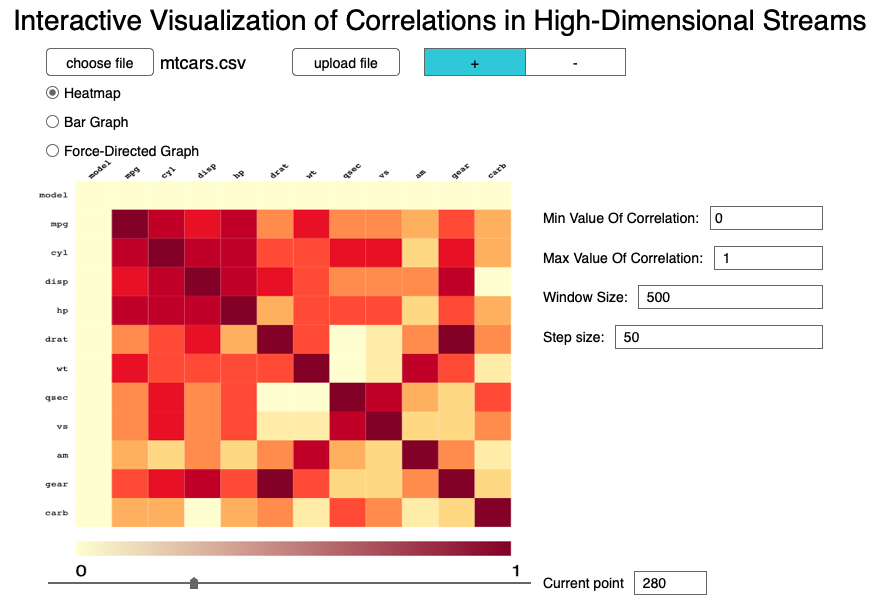
\includegraphics[width=15cm]{pictures/mockup}
	\caption{Mock-up of the interface}
	\label{fig:mockup}
\end{figure}

\section{Implementation}
\label{sec:Interface:Implementation}
As the interface is available by the web service, Javascript is the programming language for developing. In our project, we mainly use D3.js to implement the visualizations of correlations in high-dimensional data streams.
\subsection{D3.js}
\label{sec:Visualization:D3.js}
D3.js (Data-Driven Documents)\cite{D3} is a data-driven JavaScript library for producing dynamic, interactive data visualizations in web browsers. It makes use of the widely implemented SVG, HTML5, and CSS standards and allows great control over the final visual result. SVG stands for Scalable Vector Graphics which is technically an XML based markup language. It is a great tool to display icons, logos, illustrations or charts, which is supported in all major browsers and requires no third-party lib because of owning the DOM interface.\\

%What is D3.js?
%D3.js is a data-driven JavaScript library for manipulating DOM elements.
%“D3 helps you bring data to life using HTML, SVG, and CSS. D3’s emphasis on web standards gives you the full capabilities of modern browsers without tying yourself to a proprietary framework, combining powerful visualization components and a data-driven approach to DOM manipulation.” - d3js.org

%Why would You create charts with D3.js in the first place? Why not just display an image?

%Well, charts are based on information coming from third-party resources which requires dynamic visualization during render time. Also, SVG is a very powerful tool which fits well to this application case.

%The benefits of SVG
%SVG stands for Scalable Vector Graphics which is technically an XML based markup language.
%It is commonly used to draw vector graphics, specify lines and shapes or modify existing images. You can find the list of available elements here.

%Pros:
%Supported in all major browsers;
%It has DOM interface, requires no third-party lib;
%Scalable, it can maintain high resolution;
%Reduced size compared to other image formats.

%Cons:
%It can only display two-dimensional images;
%Long learning curve;
%Render may take long with compute-intensive operations.
%Despite its downsides, SVG is a great tool to display icons, logos, illustrations or in this case, charts.

\subsection{Details}
\label{sec:Visualization:Details}
The \autoref{fig:overview} is an overview of our developed interface, which is available in a browser as a web-service. Users can press the "Choose file" button to upload their own data sets.\\

\begin{figure}[h]
	\centering
	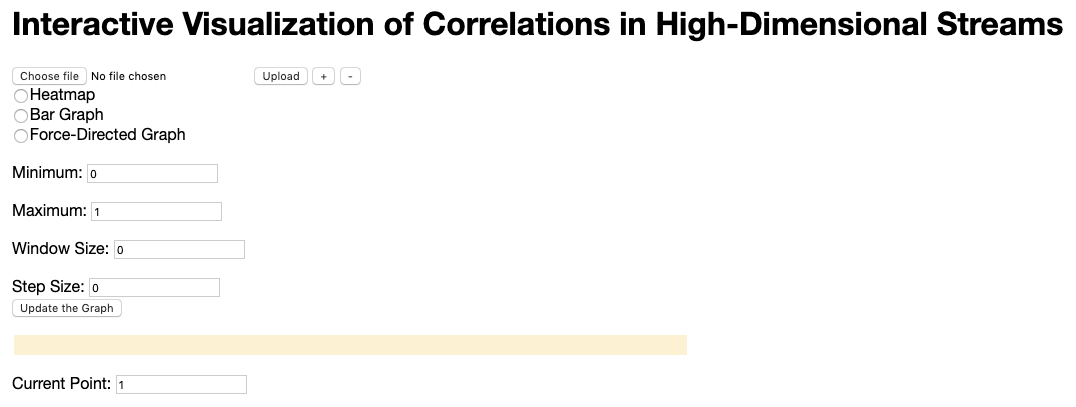
\includegraphics[width=15cm]{pictures/overview}
	\caption{Overview of the interface}
	\label{fig:overview}
\end{figure}

After pressing the \textbf{Upload} button, the data set will be stored at the back-end. The system calculates the correlations of each pair of attributes and the corresponding elements for performing the visualizations. If the calculation is finished, a confirm window will pop up to inform the maximal window size of the current data set to the user. The maximal window size is the whole size of the uploaded data. Also, the step size will be set to 1 and the window size will be set to the maximal window size after uploading the data set, see \autoref{fig:uploaded}.\\

\begin{figure}[h]
	\centering
	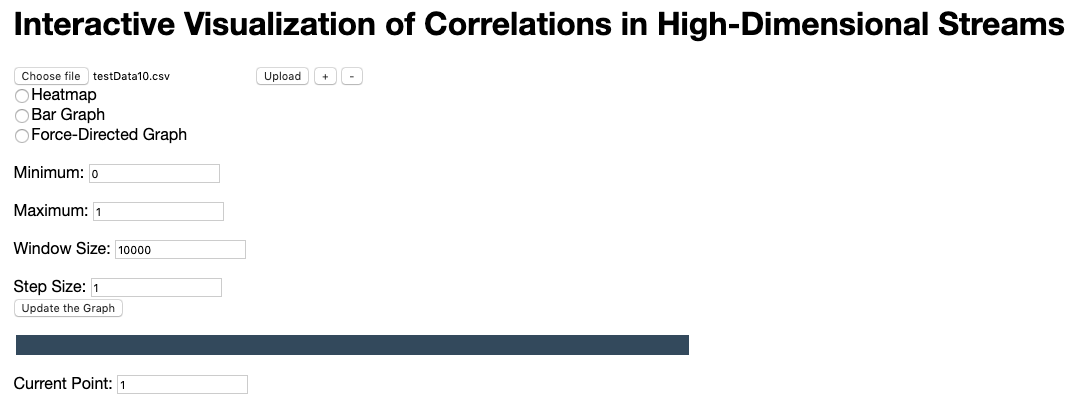
\includegraphics[width=15cm]{pictures/uploaded}
	\caption{After uploading a csv file}
	\label{fig:uploaded}
\end{figure}

Users are able to change the \textbf{minimum}, \textbf{maximum}, \textbf{window size}, \textbf{step size} and \textbf{current point}. After setting these values and pressing the \textbf{update} button, the visualization will be re-performed and the width of panel will be set to corresponding window size, seeing \autoref{fig:update}.\\

\begin{figure}[h]
	\centering
	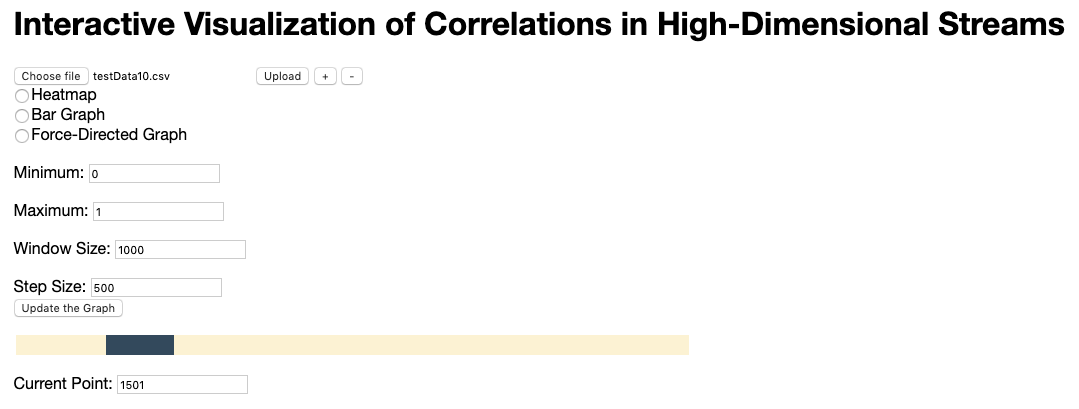
\includegraphics[width=15cm]{pictures/update}
	\caption{After pressing the "update" button}
	\label{fig:update}
\end{figure}

Our interface provides three visualization methods: Heatmap, Bar Graph and Force-Directed-Graph. After selecting the corresponding radio button, a visualization will be drawn on the web site. The \autoref{fig:choose} shows three visualizations based on the same data set we introduced in \autoref{sec:Visualization:mtcars}. \autoref{fig:chooseHM} is the Heatmap. Each box represents a pair of attributes and the color of the box represents the correlation value of this pair. \autoref{fig:chooseBar} is the Bar Graph, in which the height of each bar represents the correlation value of each pair of attributes. As 0 is not likely to be seen in case of many pairs of attributes, we paint the hole bar red and set the height to the maximal height. And \autoref{fig:chooseFDG} is the Force-Directed-Graph, in which the length of link between two nodes represents the correlation value of this pair of attributes. The shorter the linked distance is, the bigger is the correlation value. Users can also change the minimal and maximal correlation value they want to visualize, and slide the slider to see different time period of the current data set.

\begin{figure}[h]
	\centering
	\begin{subfigure}[b]{0.32\textwidth}
	\centering
	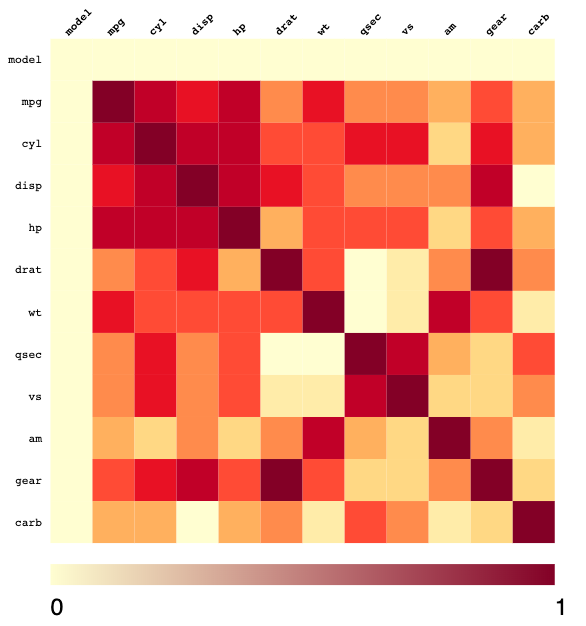
\includegraphics[width=\textwidth]{pictures/correlationMatrix}
	\caption{Select Heatmap as the visualization method}
		\label{fig:chooseHM}
\end{subfigure}
\hfill
\begin{subfigure}[b]{0.32\textwidth}
	\centering
	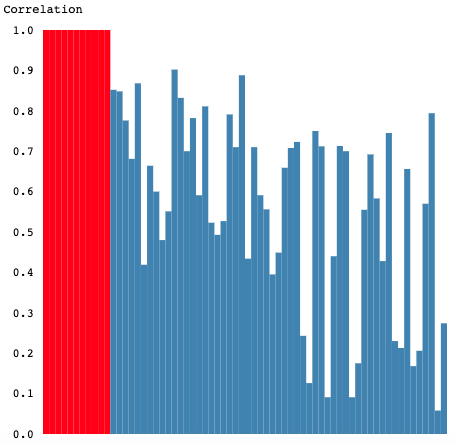
\includegraphics[width=\textwidth]{pictures/bg}
	\caption{Select Bar Graph as the visualization method}
		\label{fig:chooseBar}
\end{subfigure}
\hfill
\begin{subfigure}[b]{0.32\textwidth}
	\centering
	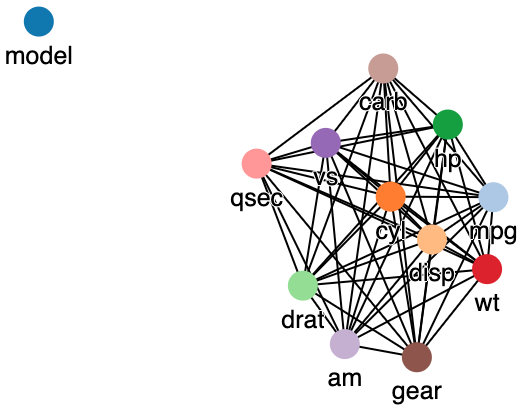
\includegraphics[width=\textwidth]{pictures/fdg}
	\caption{Select Force-Directed-Graph as the visualization method}
		\label{fig:chooseFDG}
\end{subfigure}
	\caption{Select different visualization methods}
	\label{fig:choose}
\end{figure}




%\chapter{Second Content Chapter}
%\label{ch:SecondContent}

%\dots

%\section{Second Section}
%\label{sec:SecondContent:SecondSection}

%\dots

%Add additional content chapters if required by adding new .tex files in the
%\code{sections/} directory and adding an appropriate 
%\code{\textbackslash input} statement in \code{thesis.tex}. 
%% ---------------------
%% | / Example content |
%% ---------------------
